%%%%%%%% ICML 2018 EXAMPLE LATEX SUBMISSION FILE %%%%%%%%%%%%%%%%%

\documentclass{article}

% Recommended, but optional, packages for figures and better typesetting:
\usepackage{microtype}
\usepackage{graphicx}
\usepackage{subfigure}
\usepackage{booktabs} % for professional tables

% hyperref makes hyperlinks in the resulting PDF.
% If your build breaks (sometimes temporarily if a hyperlink spans a page)
% please comment out the following usepackage line and replace
% \usepackage{icml2018} with \usepackage[nohyperref]{icml2018} above.
\usepackage{hyperref}

% Attempt to make hyperref and algorithmic work together better:
\newcommand{\theHalgorithm}{\arabic{algorithm}}

% Use the following line for the initial blind version submitted for review:
%\usepackage{icml2018}

% If accepted, instead use the following line for the camera-ready submission:
\usepackage[accepted]{icml2018}

% other packages
\usepackage{verbatim}
\usepackage{url}
\usepackage{amsmath,amssymb}

\graphicspath{ {images/} }

% The \icmltitle you define below is probably too long as a header.
% Therefore, a short form for the running title is supplied here:
\icmltitlerunning{Generalized Multi-Agent Reinforcement Learning}

\begin{document}

\twocolumn[
\icmltitle{Generalized Multi-Agent Reinforcement Learning in \\ 
	       Cooperative and Competitive Environments}

% It is OKAY to include author information, even for blind
% submissions: the style file will automatically remove it for you
% unless you've provided the [accepted] option to the icml2018
% package.

% List of affiliations: The first argument should be a (short)
% identifier you will use later to specify author affiliations
% Academic affiliations should list Department, University, City, Region, Country
% Industry affiliations should list Company, City, Region, Country

% You can specify symbols, otherwise they are numbered in order.
% Ideally, you should not use this facility. Affiliations will be numbered
% in order of appearance and this is the preferred way.
\icmlsetsymbol{equal}{*}

\begin{icmlauthorlist}
\icmlauthor{Diana Huang}{ed}
\icmlauthor{Shalini Keshavamurthy}{ed}
\icmlauthor{Nitin Viswanathan}{ed}
\end{icmlauthorlist}

\icmlaffiliation{ed}{Stanford University, Palo Alto, USA}

\icmlcorrespondingauthor{Diana Huang}{hxydiana@stanford.edu}
\icmlcorrespondingauthor{Shalini Keshavamurthy}{skmurthy@stanford.edu}
\icmlcorrespondingauthor{Nitin Viswanathan}{nviswana@stanford.edu}

% You may provide any keywords that you
% find helpful for describing your paper; these are used to populate
% the "keywords" metadata in the PDF but will not be shown in the document
\icmlkeywords{Machine Learning, ICML}

\vskip 0.3in
]

% this must go after the closing bracket ] following \twocolumn[ ...

% This command actually creates the footnote in the first column
% listing the affiliations and the copyright notice.
% The command takes one argument, which is text to display at the start of the footnote.
% The \icmlEqualContribution command is standard text for equal contribution.
% Remove it (just {}) if you do not need this facility.

%\printAffiliationsAndNotice{}  % leave blank if no need to mention equal contribution
\printAffiliationsAndNotice{\icmlEqualContribution} % otherwise use the standard text.

\begin{abstract}
Multi-agent scenarios frequently come up in the real world, but traditional reinforcement learning algorithms do not perform well on them due to constantly changing environments from the perspective of any one agent. We replicate multi-agent deep deterministic policy gradients (MADDPG), an algorithm tailored to multi-agent scenarios, and evaluate its performance in a 3-agent cooperative navigation OpenAI environment. Additionally, we perform many experiments to explore how changing hyperparameters affects performance and attempt to address the main weakness of MADDPG, which is that it does not scale well to larger numbers of agents.

Our results confirm that MADDPG performs significantly better than a single-agent policy gradient approach and show the importance of batch size in performance and training stability.
\end{abstract}


\section{Introduction}
\label{submission}

There are many applications where multiple agents need to learn how to act together, such as multiplayer games ~\cite{multigames}, multi-robot control ~\cite{multirobot}, communication scenarios ~\cite{communication}, and even self-play ~\cite{selfplay}.

Traditional reinforcement learning approaches focus on training a single agent and as a result they do not work well on multi-agent problems because the environment for any single agent changes over time as other agents change their policies, leading to instability during training and high variance in results ~\cite{unstable}. Additionally, experience replay as used with Q-learning cannot be directly applied in multi-agent scenarios, significantly hampering stable learning.

Research into multi-agent reinforcement learning has attempted to develop new approaches specifically for multi-agent scenarios. One such recently developed algorithm is multi-agent deep deterministic policy gradients algorithm (MADDPG), which obtains significantly improved results over other approaches by modifying DDPG to train agents while incorporating information from other agents \cite{maddpg}.

We replicate the MADDPG algorithm and apply it to an OpenAI cooperative navigation environment, where agents must learn to each navigate to a different fixed landmark without colliding. We experiment with various hyperparameters and exploration vs. exploitation methodologies to show how MADDPG's performance is affected by them. We also generalize MADDPG to handle larger numbers of agents and explore how performance changes accordingly.

\section{Related Work}
\subsection{Single-agent methods}
\textbf{TODO - prior work applying PG directly, Q-learning directly, etc.}

\subsection{Multi-agent methods}
\textbf{TODO - what we've read on multi-agent approaches including MADDPG}

\section{Approach}

\subsection{Environment}

We use the cooperative navigation OpenAI Gym environment for our experiments ~\cite{openaigym}. This is a 2-D world with $N$ moving agents and $N$ fixed landmarks ($N=3$ by default), where the agents must learn to each move to a different landmark while avoiding collisions with each other.

Every agent has its own state that is an 18-dimensional vector containing its own position and velocity, relative distance to each of the landmarks, and relative distance to the other agents. The action that every agent can take is represented as a 5-dimensional vector, with 4 dimensions representing movement up/down/left/right and the last dimension representing a no-move action. This is a continuous action space, with the values for each action dimension representing acceleration in a given direction.

All agents are rewarded based on the distance between landmarks and agents (the closer the agents are to separate landmarks, the higher the reward). Agents have a non-zero size, so it is possible for them to collide in this environmennt. Agents receive a reward of -1 if there are collisions at any timestep. Therefore, in order to maximize reward, the agents need to each learn to move to a different landmark while also avoiding collisions with each other.

\begin{figure}
\begin{center}
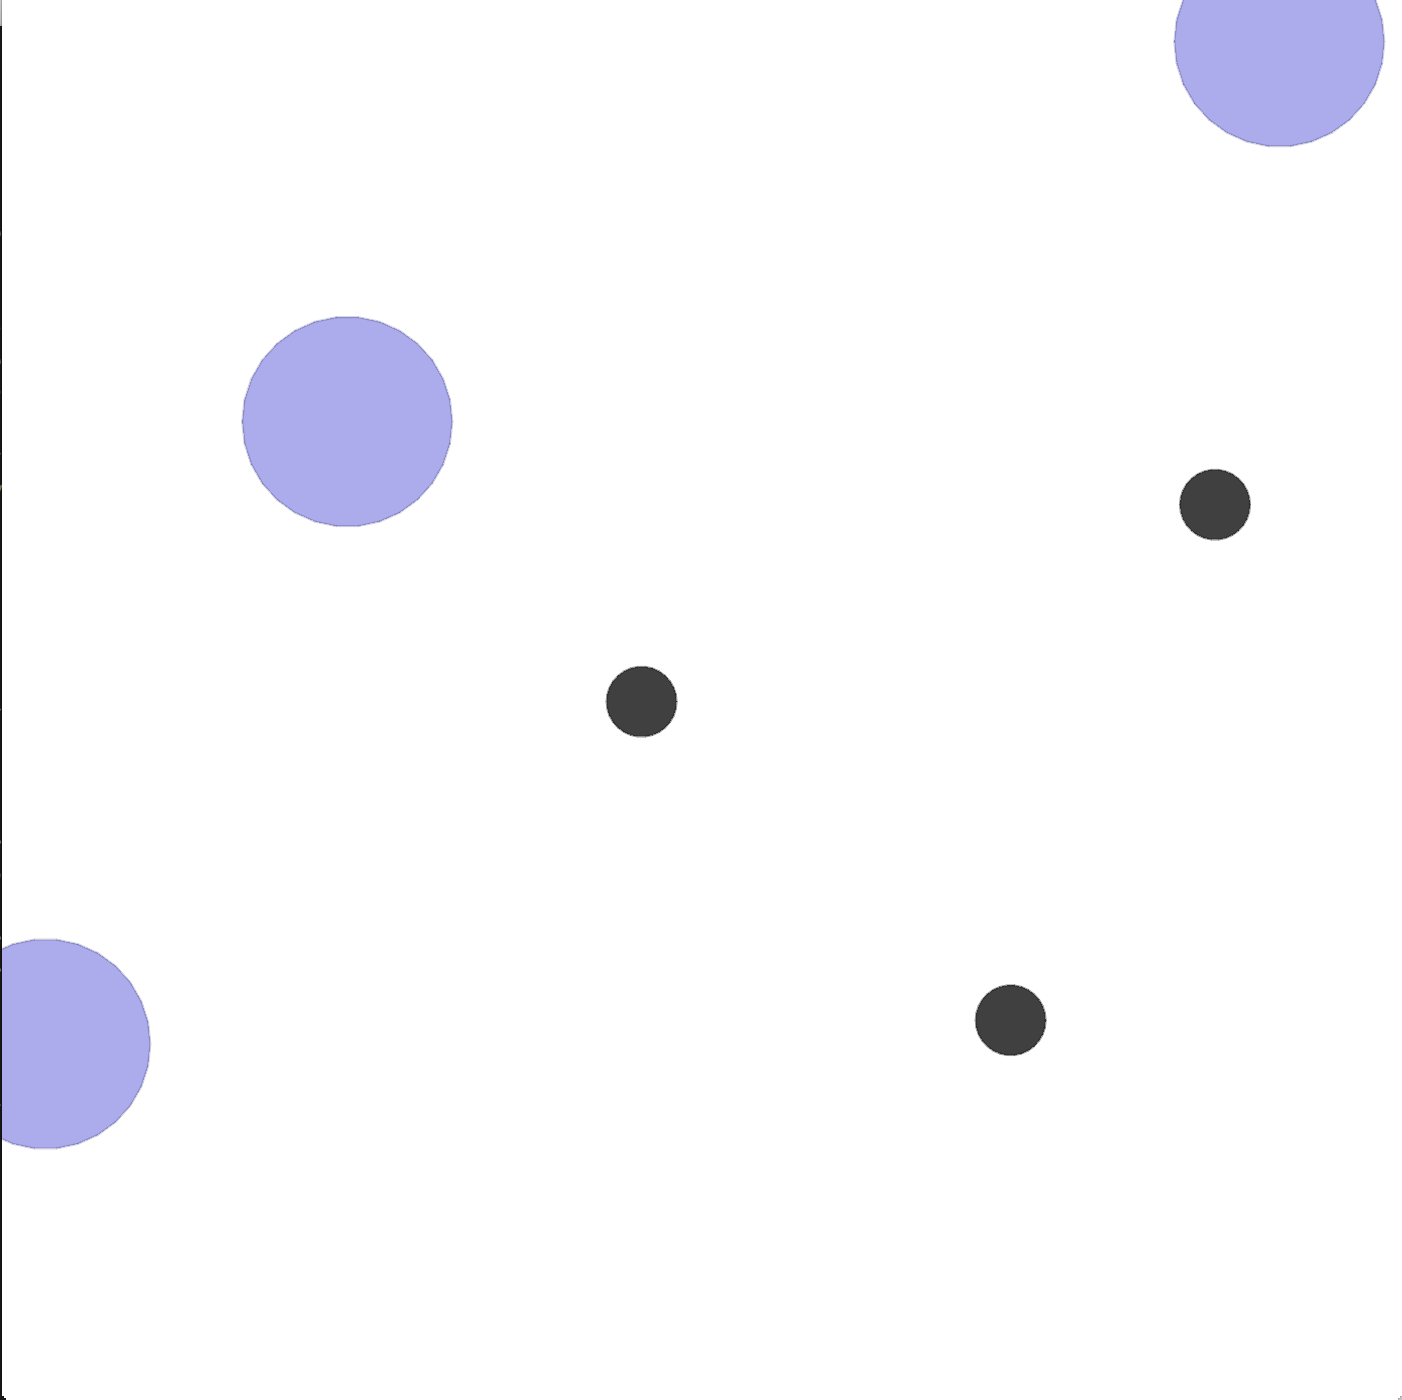
\includegraphics[scale=0.5]{env-image}
\end{center}
\caption{Cooperative navigation environment. Agents must learn to each navigate to a different landmark without colliding.}
\end{figure}

\subsection{Policy Gradient - REINFORCE}
\textbf{TODO - update}

As an initial baseline, we implement the REINFORCE algorithm for multi-agent scenarios. 

With REINFORCE and other single-agent policy gradient methods, every agent trains its own policy network based on its observation of the environment and the possible actions it can take. Even after applying a baseline and advantage normalization we did not expect REINFORCE to perform well due to the potential for very large variance in the gradient. From a single agent's perspective not only does the world change as other agents move, but the policies other agents follow change as well. Additionally, individual agents might not always get the correct gradient signal as an agent could take a good action but if other agents took bad actions, leading to overall decrease in reward, the gradient for the agent taking the correct action could still be negative. Nevertheless, REINFORCE serves as a baseline for comparing against more sophisticated approaches.

\subsection{MADDPG}
\textbf{TODO - update}

We recreate MADDPG as our main algorithm for the cooperative navigation task ~\cite{maddpg}.

MADDPG takes DDPG and tailors it to multi-agent scenarios, resulting in significantly better performance than single-agent methods such as REINFORCE and DDPG. MADDPG trains separate policy networks for every agent, but uses a centralized action-value function that incorporates information across all agents to ensure a more stable learning process. 

Consider a game with $N$ agents, and let $\pi = \{\pi_1, ..., \pi_N\}$ be the associated set of agent policies that are parametrized by $\theta_1, ..., \theta_N$. The gradient update for MADDPG for agent $i$, $\nabla_{\theta_i} J(\theta_i)$, is:

$$\nabla_{\theta_i}J(\theta_i) = \mathbb{E}_{s, a_i}[\nabla_{\theta_i}log \pi_i(a_i|o_i)Q^{\pi}_i(x, a_1, ..., a_N)]$$

Where $o_i$ is the local observation of the environment by agent $i$, $x$ is the full state information across all agents, and $Q^{\pi}_i$ is a centralized action-value function that takes as input the actions of all agents. By incorporating the actions of all agents into the action-value function, instead of only each individual agent, MADDPG produces better and more stable results than traditional policy gradient or Q-learning approaches.

\textbf{TODO - math/notes on generalizing MADDPG}

After re-implementing MADDPG, we plan to modify the original MADDPG algorithm to train agents in a generalized way. More specifically, we will still maintain a centralized critic function for each agent, but instead of taking actions from all agents as input, only actions from neighboring agents would be considered. This is to make the number of parameters in the Q network constant, rather than linear to number of agents in the environment. Thus, the computational complexity for updating the Q network is also capped.

\section{Experiments and Results}
\subsection{Evaluation Metrics}
\textbf{TODO - update}


Our primary evaluation metric has been average reward, which in this environment corresponds to the distance between agents and the target landmarks while also accounting for collisions that occur along the way. In addition to average reward, in the future we will also look at success rate, where we define success as agents successfully reaching the target landmarks with 0 collisions, no matter how long it took for this to occur. This way, we will evaluate the policy that our algorithm converges to not only based on how quickly it leads agents to reach the landmarks, but how often it leads agents to the landmarks.

\subsection{Experiments}

\textbf{TODO - include all of the various experiments we ran, and an analysis of each of them}

\textbf{TODO - also include a table with our main hyperparameters (copy from poster) and explain what they are for in text}

Figures X,Y,and Z show our initial results from training with different policy network sizes. We can see that although there is a significant improvement in average reward from the start of training, the average reward is still well below 0, indicating that the agents are not able to find an optimal strategy to cooperate and cover all of the target landmarks. This result is to be expected as policy gradient will be very unstable due to the non-stationary environment from the point of view of any given agent during training. When we increased the number of layers and units per layer we saw the network reach convergence quicker, but it was still not able to improve substantially, indicating that the algorithm itself could be a bottleneck on performance as opposed to the size of the policy networks.

\section{Conclusion}
\textbf{TODO - update}

\section{Future Work}
\textbf{TODO - update}

Apply our work to other OpenAI environments (e.g. communication and adversarial ones), explore using a modular Q function to generalize instead of a fixed number of neighbors, etc.

\section*{Contributions}
Diana wrote the initial implementation of MADDPG, Shalini wrote our logging/plotting code, and Nitin wrote the initial implementation of REINFORCE. All of us iterated on the code with bugfixes and enhancements and ran experiments using our implementations.

\bibliography{milestone}
\bibliographystyle{icml2018}

\end{document}

